\documentclass{IOS-Book-Article}

\normalfont
\usepackage[T1]{fontenc}

\usepackage[colorinlistoftodos, textwidth=4cm, shadow]{todonotes}

\usepackage{times}
\usepackage{graphicx}
\usepackage{epsfig}
\usepackage{rotating}
\usepackage{multirow}
\usepackage{amssymb}
\usepackage{pifont} 

\newcommand{\tick}{\ding{52}}

\usepackage{color}
\usepackage{listings}
\lstdefinelanguage{urdad}
{
keywords=
  {Model,ResponsibilityDomain,Query,Constraint,QualityConstraint,FunctionalRequirements,receiving,yielding,
  StateConstraint,stateAssessmentProcess,InverseConstraint,inverseOf,AndConstraint,AND,OrConstraint,OR,
  XorConstraint,XOR,from,to,many,BasicDataType,DataStructure,is,abstract,has,Variable,ofType,Constant,
  ValueOf,Exception,attribute,identification,identifying,association,linking,aggregate,component,
  QualityRequirement,requiredBy,constraint,with,constructedUsing,ResultConstraint,PreCondition,
  raises,checks,PostCondition,ensures,use,toAddress,if,ServiceContract,undoneUsing,Request,Result,
  Service,realizes,doSequential,choice,else,doConcurrent,blocking,Concurrency,wait,until,create,set,
  equalTo,add,remove,requestService,on,raiseException,returnResult,while,do,forAll,Note},%
sensitive=true,%
alsoletter={\$},%
comment=[l]{\#},%
string=[b]",%
string=[b]'%
}

%\definecolor{OliveGreen}{cmyk}{0.64,0,0.95,0.40}
%\definecolor{CadetBlue}{cmyk}{0.62,0.57,0.23,0}
\definecolor{lightgray}{gray}{0.9}
\lstset{
language=urdad,  
basicstyle=\ttfamily\tiny,
keywordstyle=\itshape\color{blue},
%keywordstyle=\color{blue},        % Keywords font ('*' = uppercase)
commentstyle=\color{gray},           
numbers=left,                           % Line nums position
numberstyle=\tiny,                      % Line-numbers fonts
stepnumber=1,                           % Step between two line-numbers
numbersep=5pt,                          % How far are line-numbers from code
backgroundcolor=\color{lightgray}, % Choose background color
frame=none,                             % A frame around the code
tabsize=2,                              % Default tab size
captionpos=b,                           % Caption-position = bottom
breaklines=true,                        % Automatic line breaking?
breakatwhitespace=false,                % Automatic breaks only at whitespace?
showspaces=false,                       % Dont make spaces visible
showtabs=false,                         % Dont make tabls visible
columns=flexible,                       % Column format
%morekeywords={__global__, __device__},  % CUDA specific keywords
}

\usepackage{color}
\usepackage{listings}
\lstdefinelanguage{pseudoCode}
{
keywords=
  {class,public,for,while,if,try,catch,return},%
sensitive=true,%
alsoletter={\$},%
comment=[l]{\#},%
string=[b]",%
string=[b]'%
}

%\definecolor{OliveGreen}{cmyk}{0.64,0,0.95,0.40}
%\definecolor{CadetBlue}{cmyk}{0.62,0.57,0.23,0}
\definecolor{lightgray}{gray}{0.9}
\lstset{
language=pseudoCode,  
basicstyle=\ttfamily\footnotesize,
keywordstyle=\itshape\color{blue},
%keywordstyle=\color{blue},        % Keywords font ('*' = uppercase)
commentstyle=\color{gray},           
numbers=left,                           % Line nums position
numberstyle=\tiny,                      % Line-numbers fonts
stepnumber=1,                           % Step between two line-numbers
numbersep=5pt,                          % How far are line-numbers from code
backgroundcolor=\color{lightgray}, % Choose background color
frame=none,                             % A frame around the code
tabsize=2,                              % Default tab size
captionpos=b,                           % Caption-position = bottom
breaklines=true,                        % Automatic line breaking?
breakatwhitespace=false,                % Automatic breaks only at whitespace?
showspaces=false,                       % Dont make spaces visible
showtabs=false,                         % Dont make tabls visible
columns=flexible,                       % Column format
%morekeywords={__global__, __device__},  % CUDA specific keywords
}

%
\begin{document}
\begin{frontmatter} 

\title{URDAD as a Quality-Driven Analysis and Design Process}
\thanks{We thank the national research foundation (NRF) of South Africa for financial support.}
\runningtitle{URDAD as Quality-Driven Methodology}
%\subtitle{Subtitle}

\author[A]{\fnms{Fritz} \snm{Solms}}
,
\author[A]{\fnms{Stefan} \snm{Gruner}}
and
\author[B]{\fnms{Cuen} \snm{Edwards}}

\runningauthor{F. Solms et al.}
\address[A]{Department of Computer Science, University of Pretoria, South Africa}
\address[B]{Solms Training and Consulting, 113 Barry Hertzog Ave, Johannesburg, South Africa}

\begin{abstract}
Use-Case Responsibility-Driven Analysis and Design (URDAD) is a service-oriented software analysis and design methodology. It is used by requirements engineers to develop technology-neutral, semi-formal platform-indepen\-dent models (PIM) within the OMG's MDA. In the past, URDAD models were denoted in UML. However, that was tedious and error-prone. The resulting models were often of rather poor quality. In this paper we introduce and discuss a new Domain-Specific Language (DSL) for URDAD. Its meta model is consistent and satisfiable. We show that URDAD DSL specifications are simpler and allow for more complete service contract specifications than their corresponding UML expressions. They also enable traceability and test case generation.
\end{abstract}

\begin{keyword}
Services-oriented design methodology\sep Model-driven development\sep Design quality\sep Model quality
\end{keyword}
\end{frontmatter}

\thispagestyle{empty}
\pagestyle{empty}

\maketitle

\section{Introduction}
Insufficiency in requirements engineering is still regarded as a root cause of poor software quality. This is due to various factors, both human and technological, including vague specification languages with only informally defined semantics. Insufficient language support for \emph{layered} specifications (i.e., decompositional system descriptions at different levels of granularity), leads software developers to making wrong presumptions about lower level requirements \cite{espana_evaluating_2009}. Tool support for the validation of requirements specifications, or for the automatic extraction of test cases from them, is also still weak \cite{bashardoust-tajali_extracting_2008}.

Model-Driven Engineering (MDE) \cite{schmidt_model_2006} aims at solving some of those problems by using modelling languages with well defined semantics, by requiring primary models to be domain models, not technical models \cite{asnina_computation_2010} and by providing tool support for MDE processes. Consequently, technology-neutral domain models are developed by requirements specialists, not by technical experts \cite{asnina_computation_2010}.

\emph{URDAD}, the Use-Case Responsibility-Driven Analysis and Design methodology \cite{fritz_solms_technology_2007} supports MDE in a service-oriented way \cite{solms_urdad_2010}. It is used by requirements specialists to develop and validate technology-neutral requirements models. URDAD models are thus Platform-Independent Models (PIM) in the Model-Driven Architecture (MDA) context \cite{solms_urdad_2010}. For each level of granularity the method leads to testable service contracts and for non-leaf services a technology neutral process realizing the service contract through the use of lower level services. Higher-level services are thus a functional composition of lower-level services, similar to the classical DFD technique \cite{demarco_tom_structured_1978}, with the levels of granularity decoupled through service contracts.

Requirements engineers have traditionally used the Unified Model Language (UML) to encode URDAD models. UML was a reasonable choice for this purpose because of its tool-supported use in the software industry. However, UML is an object oriented modeling language which is not conceptually aligned with a service oriented approach where stateless services are always assembled form lower level stateless services. On the one side it allows for a higher level services are assembled does not support many of the concepts required by the URDAD methodology explicitly and allows for a wide variety of model structures, most of which would not comply to the services-oriented structure of an URDAD model and on the other side it does not explicitly support many of the concepts required by URDAD. For example, the concept of a responsibility domain, a stakeholder, are not explicitly supported. Indeed, a specific UML \emph{profile} could be used to restrict the use of UML according to URDAD's intentions and at the same time introduce explicitly concepts required by URDAD. In practice, however, such a UML profile would contain an excessive number of metamodel constraints ensuring that a UML model complies structurally to a service-oriented URDAD model.

In this paper we present a new domain-specific language (DSL) for the domain of technology-neutral service-orien\-ted requirements modelling. Our new URDAD DSL is described in terms of a MOF/EMOF meta model. This makes it amenable to MDA tool suites for model transformations, as well as the generation of concrete textual and diagrammatic syntaxes with tool support \cite{gronback_model_2008}. To this end we analyse theoretically the modelling constructs required by URDAD. We elucidate and critically assess the URDAD meta model, and we propose a concrete textual syntax for an URDAD DSL. A Description Logics (DL)-based representation of the URDAD meta model is derived from the MOF/EMOF meta model in order to show its consistency and satisfiability.

Consequently we argue (also w.r.t. related work) that the URDAD DSL has two main advantages over the use of an URDAD UML profile. The language is considerably simpler than the UML and, with appropriate tool support, is expected to simplify the process through which requirements engineers can build high-level, technology-neutral models. Our new DSL enforces the structure required for a valid URDAD model, thereby requiring only a rather small and simple set of meta model constraints at the basis of tool-supported model validation. In addition the URDAD DSL provides better support for specifying service contracts within a service-oriented approach.



\section{Quality criteria}
\label{sec:qualityCriteria}

We use the ISO 9000:2000 \cite{hoyle_iso_2000} definition of quality stating that quality is \emph{``the degree to which a set of inherent characteristics fulfills requirements``}. For each quality requirement one can specify a quality criterion which is an observable quality characteristic of the solution and a quality measure providing a quantitative metric for the quality criterion\cite{firesmith_quality_2005}. This section identifies the stakeholders, who have an interest in the model and the process which produces the model, and discusses their specific quality criteria.

%-------------------------------------------------

\subsection{Model stakeholders and their quality criteria}
\label{sec:modelStakeholdersAndQualityRequirements}

A lot of work has already been done on defining and measuring program code quality (see, for example, \cite{boehm_barry_w._characteristics_1978}). Recently the focus has shifted onto understanding and measuring model quality \cite{lange_managing_2005,lange_improving_2006,shim_design_2008,qi_yu-dong_analysis_2010}. Though most of the work is applied to UML models, the concepts are generally applicable across analysis and design models, i.e.\ they are generally not UML specific. 

Lindland\cite{lindland_understanding_1994} provides a widely used quality categorization into \emph{semantic quality}, which assesses whether a model confers the meaning it was meant to confer, \emph{syntactic quality}, which is the degree to which the language used to specify the model conforms to the syntax rules of the language, and \emph{pragmatic quality}, which is the extent to which the model can satisfy its intended use. Christiaan Lange  \cite{lange_christiaan_assessing_2007} related model quality back to model purpose and identified a range of pragmatic model quality characteristics including complexity, traceability, modularity, completeness, consistency and communicativeness. Models that exhibit such qualities have been shown to commonly lead to systems with similar quality attributes \cite{podgorelec_estimating_2007}. In this paper we do not consider communicativeness and social quality as we feel these will be strongly influenced by both, the semantics and the model user interface(s).

The core stakeholders in the model include {\bf requirements engineering} (e.g.\ business analysis), {\bf architecture}, {\bf implementation} (e.g.\ developers), {\bf quality assurance} (e.g.\ testing), {\bf project management} and the {\bf client}. In order to address their responsibilities, these stakeholders need certain model qualities. All of these stakeholders need \emph{semantic quality} (since they need to extract the intended meaning from the model). The syntactic and pragmatic quality needs differ across stakeholders, though \emph{simplicity} and \emph{consistency} are qualities which are beneficial to all.

{\bf Requirements engineers} (e.g.\ business analysts) use the model to capture the functional and non-functional requirements of services in the form of service contracts and function (business process) designs fulfilling these service contracts. They also may use the model for validation and documentation generation, needing \emph{syntactic quality} to make this feasible.  The \emph{pragmatic qualities} particularly relevant to requirements engineers include \emph{modifiability} (as they would have to modify the model in the context of changing requirements and function improvement), \emph{simplicity} assisting understandability and modifiability, \emph{completeness} for complete requirements and function designs, model \emph{consistency}, \emph{decoupling} of functional requirements from function design, \emph{reuse} to reduce model complexity and increase model consistency, and \emph{traceability} to facilitate model validation and improve \emph{modifiability}. 

We define ``architecture'' as the infrastructure within which services are deployed and executed. Thus, whilst implementation is concerned with the actual service implementations, architecture is concerned with the infrastructure hosting the services. The architecture may span organizational, hardware and software infrastructure. Organizational and systems architects need to be able to design an architecture hosting the services in such a way that the quality criteria (\emph{quality of service}) can be met. They also need to be able to assess whether an existing architecture can host a service as per contract and specify architectural modifications if that is not the case. {\bf Architecture} typically uses the high level service contracts and function specifications. These need to be \emph{complete} and \emph{consistent}. \emph{Simplicity}, \emph{cohesion} and \emph{decoupling} make it easier for architects to obtain the required information.

Within in an MDA-based approach, {\bf implementation} (e.g.\ developers or managers who implement and control manual processes) perform the implementation mapping of the services onto an architecture specified by the architecture team. To this end, they require \emph{syntactic quality} as well as \emph{completeness} and \emph{consistency}. Furthermore, model \emph{simplicity}, \emph{decoupling}, \emph{reuse} and \emph{traceability} typically lead to implementations with those same qualities \cite{podgorelec_estimating_2007}.

The responsibility of {\bf Quality assurance} is to detect and report defects in the development process and the outputs of the process. They need the service contracts specifying both functional and quality criteria for services. \emph{Testability}, \emph{syntactic quality}, \emph{completeness} and \emph{consistency} are needed for test generation. Potential service implementations would be tested against the service contract. \emph{Traceability} is needed for impact reporting.

{\bf Project Management} uses the model for reporting and estimation purposes. \emph{Completeness} and \emph{traceability} are needed for status reporting on the implementation mapping.

The {\bf client} (business) uses the model to obtain function (business process) documentation and service contract documentation. Function (business process) documentation is useful for the general understanding and running of the system/business as well as for business process optimization. Documentation generation requires \emph{completeness}, \emph{consistency} and \emph{syntactic quality}. \emph{Decoupling} via service contracts is important to the client in the context of sourcing and assessing different concrete service providers (e.g.\ business partners, off-the-shelf systems). More generally, the client commonly needs modifiability in order to have requirements changes cost-effectively implemented, benefits from \emph{service reuse} in the context of cost containment and consistency, and needs \emph{traceability} for dependency analysis.

\begin{table}[h]
\caption{Stakeholders and their primary model quality criteria.}
\label{tab:modelQualityRequirements}
\begin{tabular}{|l|cc|cccccccc|} \hline
\multirow{4}{*}{\bf Stakeholders} & \multicolumn{10}{c|}{\bf Model quality criteria} \\ \cline{2-11}
& & & \multicolumn{8}{c|}{Pragmatic model quality criteria}\\ \cline{4-11}
    & \begin{sideways}Semantic\end{sideways} & \begin{sideways}Syntactic\end{sideways}  & \begin{sideways}Simplicity\end{sideways}
    & \begin{sideways}Completeness\end{sideways} & \begin{sideways}Modifiability\end{sideways} & \begin{sideways}Consistency\end{sideways}
    & \begin{sideways}Decoupling\end{sideways} & \begin{sideways}Cohesion\end{sideways} & \begin{sideways}Reusability\end{sideways}
    & \begin{sideways}Traceability\end{sideways} \\ \hline
%                         Semantic     Syntax        Simplicity  Completeness   Modifiable  Consistent  Decoupled    Cohesion     Reuse        Traceable
Requirements engineering & \checkmark & \checkmark & \checkmark & \checkmark & \checkmark & \checkmark & \checkmark & \checkmark & \checkmark & \checkmark \\
Architecture             & \checkmark &            & \checkmark & \checkmark &            & \checkmark & \checkmark & \checkmark &            &       \\ 
Implementation           & \checkmark & \checkmark & \checkmark & \checkmark &            & \checkmark & \checkmark & \checkmark & \checkmark & \checkmark \\ 
Quality assurance        & \checkmark & \checkmark & \checkmark & \checkmark &            & \checkmark &            &       &            & \checkmark \\ 
Project management       & \checkmark &            & \checkmark & \checkmark &            & \checkmark &            &       &            & \checkmark \\ 
Client (business)        & \checkmark & \checkmark & \checkmark & \checkmark & \checkmark & \checkmark & \checkmark &            & \checkmark & \checkmark \\ \hline
\end{tabular}
\end{table}

%---------------------------------------------------------------------------------------------------------%

\subsection{Process stakeholders and their quality criteria}

The {\emph Capability Maturity Model} (CMM) \cite{paulk_capability_1993} defines a range of quality attributes for mature processes including \emph{process definition}, \emph{measurability}, \emph{trainability}, \emph{repeatability} and at the higher level the ability to continuously optimize processes for \emph{cost} and other qualities. Berard\cite{berard_what_1995} discusses a related set of general requirements for a methodology including \emph{repeatability}, \emph{trainability}, \emph{wide process applicability}, and quality improvement in the outputs of the methodology. 

{\bf Project management} needs to perform planning, estimation, resource management, monitoring, control and reporting during the analysis and design process. To this end, they need \emph{estimatability}, \emph{repeatability} for accurate estimation and \emph{measurably} and tool support facilitating estimation, monitoring, and reporting.

{\bf Requirements engineers} execute the process itself generating the analysis and design model. They requires a process which is \emph{usable} and \emph{trainable}, and \emph{repeatable}.

The {\bf client} (e.g.\ business) requires \emph{low process cost}, a \emph{trainable} process, enabling the client to easily train up additional requirements engineers, and \emph{isolation}. Process isolation refers here to the ability to grow islands of expertise around the process, extracting value from those teams which apply the process without requiring that the process needs to be rolled out either across an entire project team or across an entire organization. This enables the client to take a risk-averse, incremental approach which allows for customization and controlled, incremental roll-out.

A further property required of a process is internal consistency. This property will be discussed in section \ref{sec:urdadConsistency}.

\begin{table}[h]
\caption{Stakeholders and their primary process quality criteria.}
\label{tab:processQualityRequirements}
\begin{tabular}{|l|ccccccc|} \hline
\multirow{2}{*}{\bf Stakeholders} & \multicolumn{7}{c|}{\bf Process qualities} \\ \cline{2-8}
    & \begin{sideways}Low cost\end{sideways}  & \begin{sideways}Repeatability\end{sideways} & \begin{sideways}Estimatability\end{sideways}
    & \begin{sideways}Trainable\end{sideways}
    & \begin{sideways}Measurability\end{sideways} & \begin{sideways}Consistency\end{sideways} & \begin{sideways}Isolation\end{sideways} \\ \hline
%                          Cost         Repatable    Estimatable  Trainable    Measurable  Consistent   Isolated
Project management       &            & \checkmark & \checkmark & \checkmark &            & \checkmark & \checkmark \\
Requirements engineering & \checkmark & \checkmark & \checkmark & \checkmark & \checkmark & \checkmark & \checkmark \\
Client (business)        & \checkmark & \checkmark & \checkmark & \checkmark & \checkmark & \checkmark \\ \hline
\end{tabular}
\end{table}


\section{Quality drivers}
\label{sec:qualityDrivers}

A quality drivers is defined as an activity which improves one or more process or model quality criteria\cite{petersen_software_1989}. The relience on quality-drivers forms the basis for the concept of a \emph{`quality-driven'} process. In this section we look at each model and process quality criterion and discuss activities (quality drivers) which can be used to improve the quality criterion. The list of quality-drivers presented here is not intended to be exhaustive but includesrepresents a collection of quality-drivers which are widely known and used. In addition to identifying quality-drivers, we also note that quality metrics can be applied to the resultant model in order to assess model quality. This section discusses some commonly used quality metrics for the identified quality criteria suitable for a service-oriented approach. For a more general list of model quality metrics the reader should consult \cite{mohagheghi_existing_2009}.

\subsection{Model quality drivers}

\emph{Semantic Model Quality} relates to semantic accuracy and completeness. It is influenced by the quality of the modeling language and hence by the semantic quality of the metamodel of the modeling language. The latter is determined by its semantic completeness, consistency and complexity\cite{buder_effects_2010}. Semantic completeness refers to the power of the formal language to express all propositions. More precisesly, a formal system is said to be semantically complete if and only if every theorem of the system is provable in the system.  A core semantic quality-driver is thus the specification of a metamodel for the analysis and design model which itself is shown to be semantically complete and consistent.

\emph{Syntactic Quality} elates to correct language usage\cite{lange_christiaan_assessing_2007}, i.e.\ that the grammatical statements made comply to the abstract syntax as specified via the metamodel and its constraints or an ontology and its associated rules. A commonly used syntactic quality driver is the definition of concrete text and/or graphical grammars and a transformation between the concrete and abstract syntax. Models which are defined through and verified against the concrete syntax can be shown to comply to the abstract syntax of the associated metamodel. Editors generated from the concrete syntax definition generally validate syntactic correctness. In this paper we confine the assessment of syntactic quality to the existence of a formal modeling language and concrete grammar for model specification. We will thus assume that model instances will adhere to the grammar of the chosen modeling language as this can easily be verified.

\emph{Simplicity} is the inverse of complexity. The complexity of the modeling language is usually assessed by measuring the complexity of the metamodel for that language\cite{mohagheghi_evaluating_2007}. A lot of work has been done on model complexity itself. Common approaches include using information entropy measures\cite{abrahamsson_extreme_2004}, language-theoretic approaches\cite{podgorelec_estimating_2007} and function complexity assessment based on the McCabe complexity measure \cite{mccabe_complexity_1976}. A service-oriented approach already enforces certain drivers for simplicity. In particular it enforces the assembling of functions from independent, stateless services, the enforced decoupling through services contracts, the improved reuse through the implied service discovery, as well as an implied adapter layer facilitating reuse across technologies and interfaces mismatches. A metamodel confining the modeling constructs and relationships between these, as well as a convenient grammar, reduce complexity. Another core driver for simplicity is the decomposition across levels of granularity enabling the understanding and processing of one level of granularity before having to concern oneself with the details of the next lower level of granularity. The availability of a services contract enables one to look at a service from a user/service consumer perspective before understanding the service function. Finally, traceability links and in particular enforced satisfaction links (i.e.\ that a functions may only use services which address functional requirements of the service) are drivers for simplicity.

\emph{Completeness} of requirements is difficult to assess, though the discovery of certain stakeholders for which no functional or non-functional requirements exist is an indication of missing requirements. Design completeness is easier to assess as there is a global point of reference - the degree to which the requirements are fulfilled. Core quality-drivers for completeness include enforced satisfaction links, the enforcement of testable pre- and post-conditions, as well as having a metamodel which enforces certain content, either structurally, or through metamodel constraints. In a service-oriented approach, a completeness metric can be specified as a function of 1) the percentage of functional requirements not addressed in the designed functions (identified through missing satisfaction links)\cite{shim_design_2008}, 2) the fraction of pre- and post-conditions for which the test process has not been specified and 3) the percentage of request and result classes for which the data structures have not been specified. At the implementation level completeness can be assessed as the fraction of services for which service implementations are not yet available.

\emph{Consistency} is an important model property. A lot of emphasis has been placed on model consistency for UML models. This is so because UML models are often inconsistent due to the multi-diagram approach and the complexity of the modeling language itself\cite{lange_empirical_2004}. A commonly quality-driver for model consistency is to use a much smaller (less general) language with more formally defined semantics which enforces the consistency through both, its structure and a set of metamodel constraints.

\emph{Cohesion} in a service-oriented approach has been extensively studied by Mikhael Perepletchikov et al.\ \cite{perepletchikov_cohesion_2007,perepletchikov_impact_2010}. Their approach is closely related to that of unity criteria \cite{gonzalez_unity_2009} identifying and quantifying interfacing cohesion, usage cohesion and implementation cohesion. These cohesion measures can be applied directly to an URDAD model. Quality-drivers for cohesion include enforcing the single responsibility principle as well as localizing all controll and decision logic for a service in a controller service. 

\emph{Decoupling} is enforced in a service-oriented approach by requiring that services are only consumed via services contracts. This decouples services across levels of granularity. Quality-drivers for decoupling include a metamodel which enforces contracts based decoupling through metamodel structure and localization of function logic within a controller. The latter ensures that lower level services remain decoupled, i.e.\ that they do not call each other. In a service-oriented architecture, the number of services which are directly coupled to concrete lower level services can be used as a measure of coupling\cite{shim_design_2008}.

\emph{Modifiability} refers to the efficiency with which model changes can be applied, i.e.\ it is related to the inverse of the cost required to make model changes. Modifiability is difficult to quantitatively measure. It is supported by other model qualities like \emph{simplicity},  \emph{decoupling} (modifiability through pluggability), and \emph{cohesion} (localized maintenance). A further quality-driver in the form of localizing function logic within a controller service, thereby projecting out additional levels of granularity. Shim et al.\ \cite{shim_design_2008} define a quality metric for modifiability (flexibility) of service-oriented designs as a weighted sum of coupling, service granularity, and parameter granularity. Since increased complexity and coupling reduce modifiability, the quality drivers for simplicity and decoupling are also quality drivers for modifiability.

\emph{Reusability} provides a measure of the ability and likelihood that a service can be reused. Khoshkbarforoushha et al.\  \cite{khoshkbarforoushha_metric_2010,choi_quality_2008,feuerlicht_determinants_2007}
\cite{khoshkbarforoushha_metric_2010} point out that service reusability is often caused by contract and requirements mismatch. The former can be addressed via adapters. Core quality-drivers for reusability include \emph{decoupling} via services contracts with the latter also driving discoverability and consumability, \emph{levels of granularity} via process localization within a reusable controller service, and \emph{cohesion} through enforcing the single responsibility principle. Indeed, \cite{shim_design_2008} defines a simple quantitative reusability measure for service-oriented systems as a weighted sum of coupling, cohesion, granularity, and consumability.

\emph{Traceability} is needed for design validation and estimation. Validation includes assessing sufficiency and necessity. Ramesh and Jarke \cite{ramesh_toward_2001} identify four types of traceability links in models including \emph{satisfaction} links used to assess whether requirements are satisfied, \emph{evolutionary} links to trace along the evolution of an artifact over time, \emph{rationale} links which typically link requirements to higher level business goals, and \emph{dependency} links enabling one to identify dependencies of model elements. Quality-drivers include thus the availability of these traceability links in the modeling language and their enforced usage through the modeling process.

\section{URDAD}

\begin{itemize}
  \item Modeling in problem domain
  \item sevices-oriented analysis and design methodology
  \item contract focused
  \item Responsibility driven
  \item semi-formal (agile/formal)
  \item levels of granularity
  \item
\end{itemize}


\section{Discussion of quality drivers used by URDAD}

The model and process quality drivers discussed in \ref{sec:modelQualityDriversAndMetrics} are built into the URDAD process. Table \ref{tab:qualityDrivers} lists the employed model quality drivers and the model qualities they are meant to support.

\begin{table}[h]
 \caption{URDAD model quality drivers related to model qualities.}
 \label{tab:qualityDrivers}
\begin{tabular}{|l|cc|cccccccc|} \hline
\multirow{4}{*}{\bf Quality-driver} & \multicolumn{10}{c|}{\bf Model qualities} \\ \cline{2-11}
& & & \multicolumn{8}{c|}{Pragmatic model qualities}\\ \cline{4-11}
    & \begin{sideways}Semantic\end{sideways} & \begin{sideways}Syntactic\end{sideways}  & \begin{sideways}Simplicity\end{sideways}
    & \begin{sideways}Completeness\end{sideways} & \begin{sideways}Modifiability\end{sideways} & \begin{sideways}Consistency\end{sideways}
    & \begin{sideways}Decoupling\end{sideways} & \begin{sideways}Cohesion\end{sideways} & \begin{sideways}Reusability\end{sideways}
    & \begin{sideways}Traceability\end{sideways} \\ \hline
%                                       Semantic     Syntax        Simplicity  Completeness   Modifiable  Consistent  Decoupled    Cohesion     Reuse        Traceable
Define metamodel or ontology                   & \checkmark & \checkmark & \checkmark & \checkmark & \checkmark & \checkmark & \checkmark &            &            & \checkmark \\
Define concrete DSL grammars                   &            & \checkmark & \checkmark &            & \checkmark &            &            &            &            
& \\
Fix levels of granularity                      &            &            & \checkmark &            & \checkmark &            &            &            &
\checkmark & \checkmark \\ 
Decouple services via contracts                &            &            & \checkmark &            & \checkmark &            & \checkmark &            & \checkmark & \checkmark \\ 
Apply single reponsibility principle           &            &            & \checkmark &            & \checkmark &            &            & \checkmark & \checkmark & \checkmark \\ 
Specify testable pre- \& post-conditions       &            &            &            & \checkmark & \checkmark & \checkmark &            &            &            &  \\ 
Localize process within controller             &            &            & \checkmark &            & \checkmark &            & \checkmark & \checkmark & \checkmark & \checkmark \\ 
Include traceability Links                     &            &            & \checkmark & \checkmark & \checkmark & \checkmark &            &            &            & \checkmark \\ \hline 
\end{tabular}
\end{table}

The \paragraph{semantic quality} has been verified through analyzing the URDAD process and models for the set of statements required by the URDAD methodology and checking that each of the required statements can be made using the URDAD DSL. The URDAD metamodel has also been empirically tested by encoding example models and verifying analytically whether all the information required for code and test generation is available from the model. The consistency of the URDAD metamodel has been verified by transforming the metamodel to an ontology using the \emph{TwoUse} \cite{parreiras_using_2010} Eclipse plugin and analysing the ontology with respect to consistency using a description logic reasoner. The complexity of the modeling language was constrained by including only concepts required by the URDAD methodology. The URDAD metamodel has about an order of magnitude less classes and realationships than the UML.

\paragraph{Syntactic quality} is enforced by having a concrete text syntax specified for the URDAD DSL. A concrete diagrammatic syntax is currently being developed. We have also generated a syntax-validating compiler for the concrete text syntax which enforces adherence of the model specification to the URDAD DSL text grammar. In addition we use validators to assess adherence to the URDAD metamodel structure and compliance with the URDAD metamodel constraints.

\paragraph{Reusability Drivers} employed by URDAD include the requirement that all services must realize a service contract and hence be pluggable. Furthermore, the process includes a step checking whether any of the required services can be combined into a single, cohesive, higher level service, resulting in improved reusability across levels of granularity. Cohesion and hence its quality drivers also improve discoverability and reusability. Linkage between service and contract it realizes aids service provider discoverability. The URDAD process is a technology neutral process assembling processes from services specified through services contracts. During the implementation mapping phase an adapter layer is inserted which adapts concrete service providers to the service contract further improving reuse.

The quality drivers used for \paragraph{simplicity} include the specification of  the URDAD DSL which provides a compact, precise language for URDAD which reduces model size and improves model understandability when compared to using the UML. The process also enforces that all activities specified for the realization of a service are activities which address functional requirements. Enforcing the \emph{single responsibility principle} improves simplicity through separation of concerns. Furthermore, the process includes a step checking whether any of the required services into a single, cohesive, higher level service, resulting in improved reusability across levels of granularity. The URDAD metamodel also does not allow for duplicate process specification, When using the UML a process can be specified through a variety of diagrams including activity and sequence diagrams, state charts, collaboration diagams and even interaction overview diagrams. The extensive notation, potential information duplication and inconsistency risks all add to model complexity.

The quality drivers used for \paragraph{cohesion} include that the process assigns services contracts to responsibility domains. Enforcing services to be stateless, i.e.\ that no state is maintained within a service across service requests, makes services self-contained, cohesive units of functionality.

Model \paragraph{consistency} across UML models is generally very weak - different UML models have commonly very different model structures and are often even semantically different. Furthermore, using different diagrams, particularly for process specification, commonly results in inconsistency issues across these diagrams. The model consistency drivers used within the URDAD include that the specification of a metamodel which fixes the model structure of an URDAD model. Furthermore the process specifies a set of process steps with defined inputs, outputs and activities for each process step.

Structural model \paragraph{completeness} is enforced through the metamodel. Process completeness is partially addressed by requiring that the process must include activities which address all functional requirements. The process does not, however, enforce completeness over levels of granularity. A model is regarded as complete if a level of granularity is complete. This makes the assumption that service providers realizing the services contracts for the required services can be found. URDAD does not verify the latter.

\paragraph{Modifiability} is addressed through enforced decoupling via services contracts, localization of process definition. The defined levels of granularity also improve modifiability because modifications often have to only ba applied to a particular level of granularity. The enforced usage of stateless services improves modifiability because it leads to the ability to easily assemble new processes and modify existing processes. Simplicity and hence its quality drivers also improve modifiability.

\paragraph{Traceability} is important for validation and estimation. URDAD facilitates traceability through the process requiring to identify the service to be used to address each functional requirement. The metamodel provides traceability of services across levels of granularity,  from services to the functional requirement realized and from a functional requirement to the stakeholder who requires it.

The process quality drivers employed by URDAD are shown in table \ref{tab:processQualityDrivers}

\begin{table}[h]
\caption{URDAD model quality drivers related to model qualities.}
\label{tab:processQualityDrivers}
\begin{tabular}{|l|ccccccc|} \hline
\multirow{2}{*}{\bf Quality-driver} & \multicolumn{7}{c|}{\bf Process qualities} \\ \cline{2-8}
    & \begin{sideways}Low cost\end{sideways}  & \begin{sideways}Repeatability\end{sideways} & \begin{sideways}Estimatability\end{sideways}
    & \begin{sideways}Trainable\end{sideways}
    & \begin{sideways}Measurability\end{sideways} & \begin{sideways}Consistency\end{sideways} & \begin{sideways}Isolation\end{sideways} \\ \hline
%                    Cost         Repeatable    Estimatable  Trainable    Measurable  Consistent   Isolated
Simple             & \checkmark & \checkmark &            & \checkmark &            &            &            \\
Process definition & \checkmark & \checkmark &            & \checkmark & \checkmark & \checkmark &            \\
Decoupling         &            &            &            &            &            &            & \checkmark \\ 
Metrics            &            &            & \checkmark &            & \checkmark &            &            \\ 
Recursive process  &            & \checkmark &            & \checkmark &            & \checkmark & \checkmark \\ \hline
\end{tabular}
\end{table}



%\section{Internal consistency of the URDAD methodology}
\label{sec:urdadConsistency}

URDAD is an analysis and design methodology used to design services. If one uses the methodology to design a service for analyzing the services contract and designing a technology neutral process for a service, the constructed model should be a model for URDAD, containing the URDAD process as the service process and the URDAD metamodel for the domain concepts. If this is not the case then URDAD would be inconsistent because it would state ``use this methodology to design services, but use something else/better to design the service for designing a service''.
      \begin{itemize}
		  \item Apply process to design service of performing analysis \& design for service.
			 \begin{itemize}
				\item Should result in service with process, semantics \& model structure which represents URDAD itself.
				\item If it doesn't, then not internally consistent.
            \item If it does, it does not show that URDAD is a good methodology, but only that it is consistent.
In order to validate the internal consistency of the URDAD methodology, we used URDAD to design the service of performing a services-oriented analysis and design. If the methodology is consistent it needs to either regenerate itself or at least something which is largely equivalent to itself. It would, of course, not follow that URDAD is a ``good'' methodology, only that it is a consistent methodology.

Due to space constraints we cannot go through the full process across levels of granularity. Instead we demonstrate the consistency by looking at a particular level of granularity and point out how URDAD starts regenerating itself as process and how its own metamodel is regenerated. We also use this opportunity to show aspects of the URDAD metamodel and the text grammar of the URDAD-DSL\footnote{A separate paper discussing the URDAD metamodel and domain specific language for URDAD is currently being reviewed.}. To make this more interesting we omit the first level of granularity which is a process which contains the analysis and process design steps for a particular level of granularity. We zoom directly into the \emph{performAnalysis} service which has more interesting pre- and post-conditions and consequently a more interesting process specification.

\begin{figure}[Htbp]
  \centering
  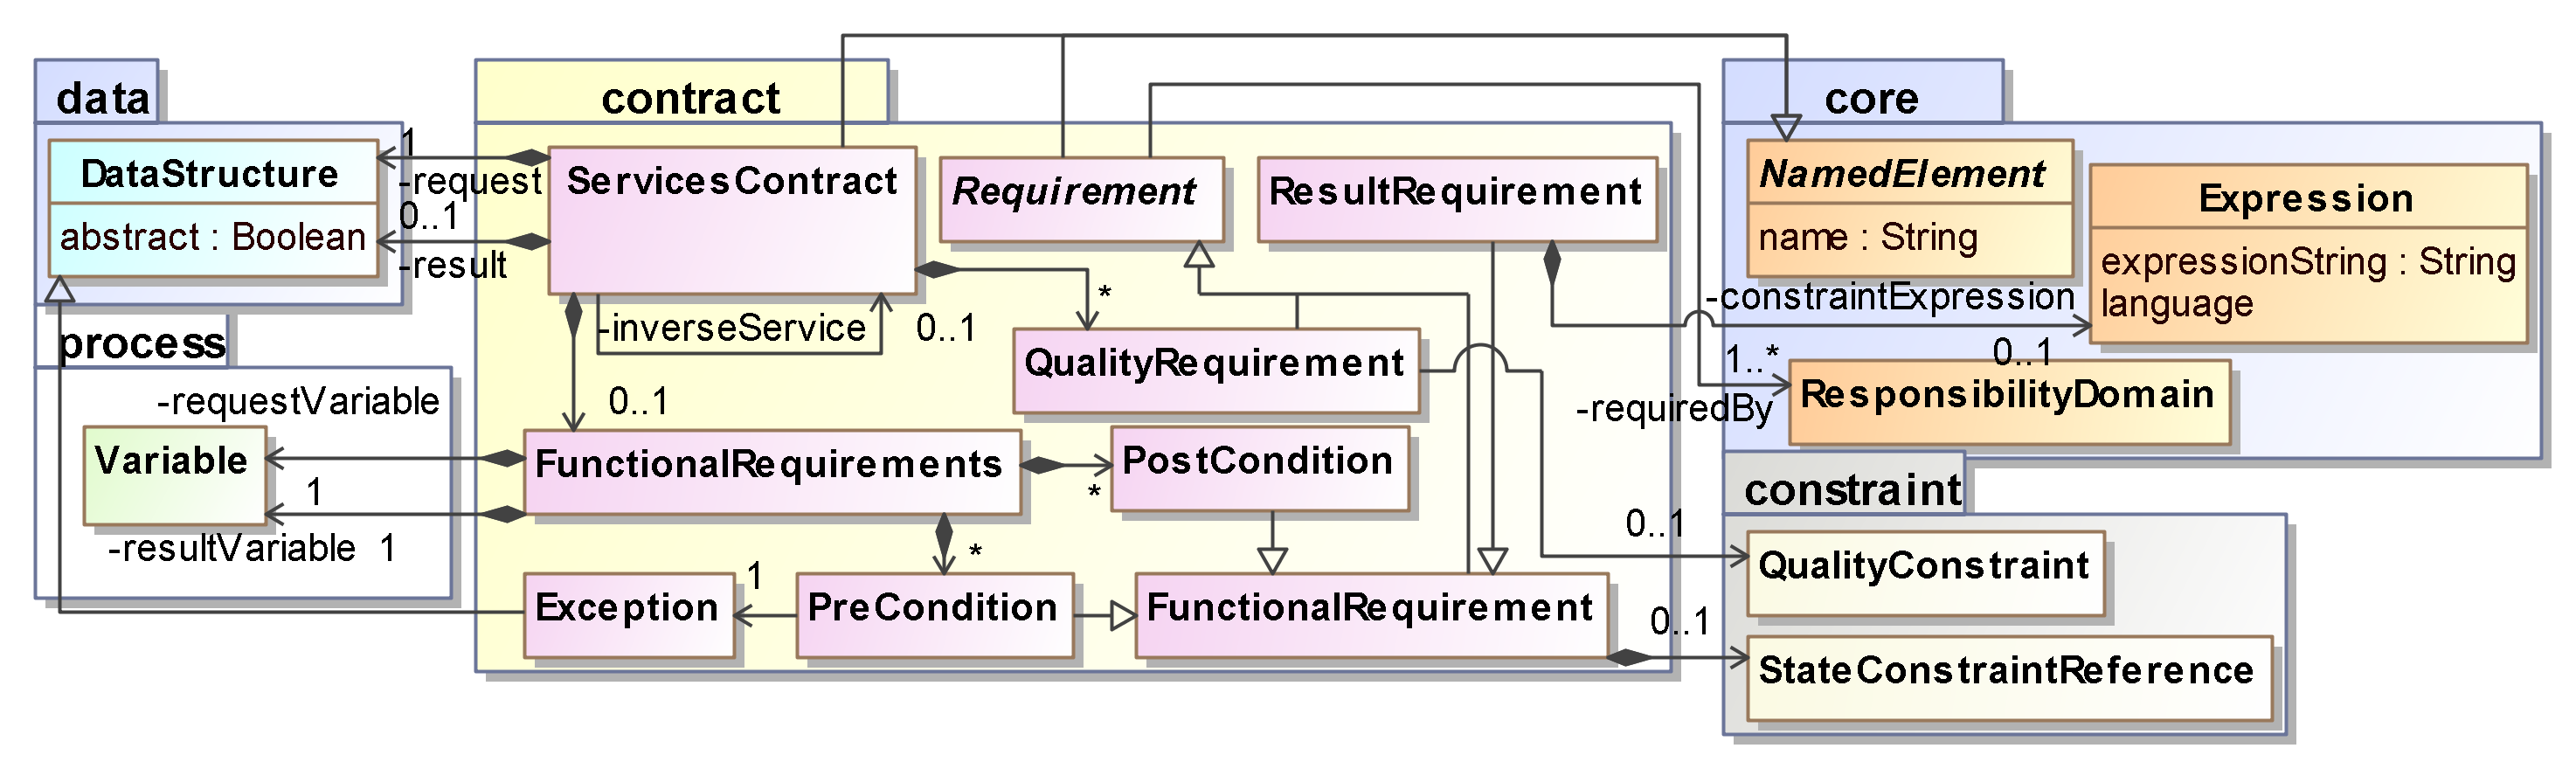
\includegraphics{contract}
  \caption{The modeling constructs available in URDAD introducing the semantics for services contracts}
  \label{fig:contractModule}
\end{figure}

We start by eliciting the stakeholders (yielding the stakeholders identified in section \ref{sec:qualityCriteria}) and their functional requirements. The output is a service contract specification for the \emph{performAnalysis} service which itself contains the concept of a service contract. The URDAD metamodel support for service contract specification is shown in figure \ref{fig:contractModule}. Below we use the text grammar defined for the URDAD-DSL to specify the service contract for the \emph{performAnalysis} service:

\lstset{language=urdad,caption=Specifying a state constraint in the URDAD text grammar.,label=contractTextSyntax}
\begin{lstlisting}[numbers=left,escapechar=|]

ResponsibilityDomain RequirementsEngineering
{
  ServiceContract provideService
  {
    FunctionalRequirements receiving Variable provideServiceRequest ofType ProvideServiceRequest yielding Variable provideServiceResult ofType ProvideServiceResult
    {
      PreCondition serviceHasStakeholders requiredBy (Client) raises NoStakeholdersException checks Constraint ServiceHasStakeholders
      PreCondition stakeholderRequirementsConsistent requiredBy (Client Implementation Testing) raises InconsistentStakeholderRequirementsException checks Constraint RequirementsConsistent
      PostCondition serviceContractSpecified requiredBy (Implementation Testing) ensures Constraint ServiceContractSpecified
      PostCondition serviceSourcedFromEnvironment if Constraint ServiceAvailable requiredBy (Client) ensures Constraint ServiceSourced with Query OCL:"serviceContract"
      PostCondition serviceSpecified if Constraint Not ServiceAvailable requiredBy(Client Implementation) ensures ServiceSpecified
      QualityRequirement traceability requiredBy (ProcessDesign ProjectManagement Development)  
    }
    Request DataStructure ProvideServiceRequest
    {
       has Component serviceRequirements ofType _ServiceRequirements
    }
    Result DataStructure ProvideServiceResult
    {
      has Component serviceContract ofType _ServiceContract
      has Component service ofType _Service
    }        
  }
  ...
} 
\end{lstlisting}

Note how we are already regenerating the URDAD metamodel in that the \verb+ServiceContract+ for perform analysis generates a domain which includes the concept of a \verb+_ServiceContract+. As we follow the URDAD methodology to design itself, we traverse levels of granularity, incrementally generating lower level aspects of the URDAD process and the URDAD metamodel, populating the finer details in the metamodel classes and the lower level process elements of the URDAD process. Throughout the classes without underscore prefix are the metamodel classes whilst the classes with underscore prefix are the classes generated by the methodology itself. 

\lstset{language=urdad,caption=Regenerated metamodel classes.,label=constraintTextSyntax}
\begin{lstlisting}[numbers=left,escapechar=|]
DataStructure _ServiceContract 
{
    has Component functionalRequirements ofType _FunctionalRequirements
    has Component request ofType _DataStructure
    has Component result ofType _DataStructure
}
\end{lstlisting}

\begin{figure}[Htbp]
  \centering
  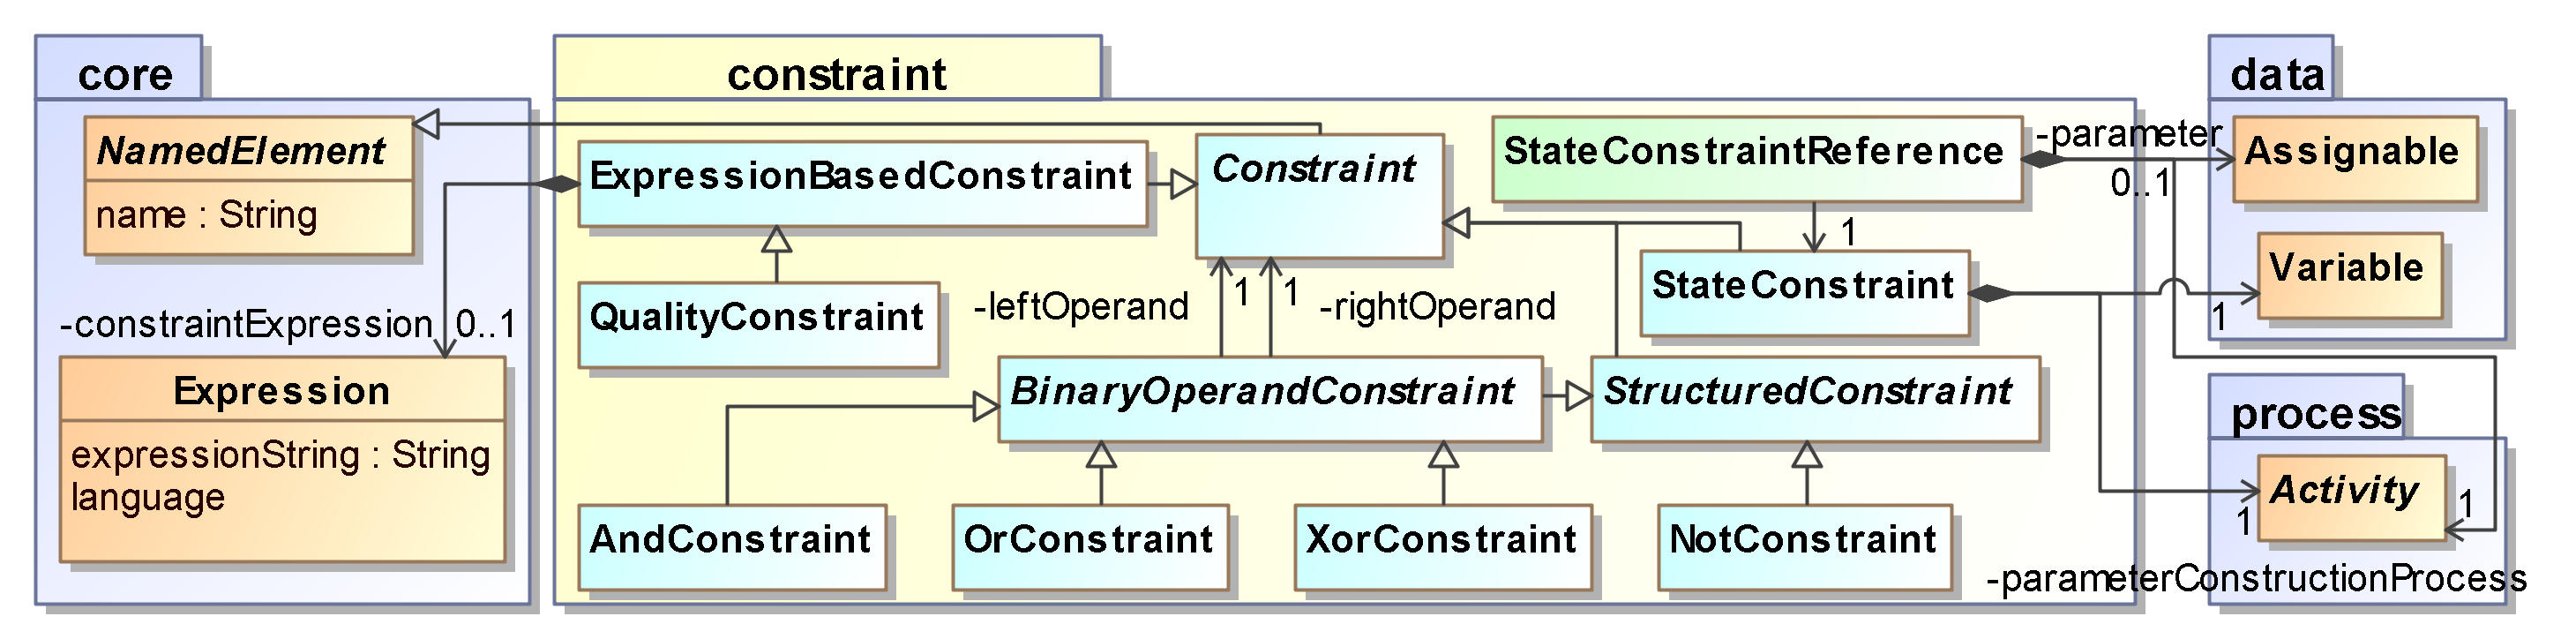
\includegraphics{constraint}
  \caption{The modeling constructs available in URDAD facilitating the specification of constraints.}
  \label{fig:constraintModule}
\end{figure}

Service contracts refers to reusable, parametrized state constraints. Figure \ref{fig:constraintModule}, shows URDAD's modeling elements for specifying such constraints. In a separate paper currently under review we have pointed out that the Object-Constraint Language (OCL)\cite{_object_2010}  alone is not expressive enough to specify reusable, parametrized constraints for a services oriented approach where one needs to extract information from the environment via services and then apply data structure constraints on the obtained environmental information.

The following listing shows an simple example of a parametrized constraint, \emph{ServiceHasStakeholders}, which demonstrated that a state constraint is assembled from a process that extracts information from the environment and a set of data constraints applied to the obtained information.
\lstset{language=urdad,caption=Specifying a state constraint in the URDAD text grammar.,label=processTextSyntax}
\begin{lstlisting}[numbers=left,escapechar=|]
StateConstraint ServiceHasStakeholders receiving Variable serviceRequirements ofType _ServiceRequirements 
{
  StateAssessmentProcess doSequential 
  {
    create Variable identifyStakeholdersRequest ofType IdentifyStakeholdersRequest
    set Query OCL:"identifyStakeholdersRequest.serviceRequirements" equalTo Query OCL:"serviceRequirements"
    requestService identifyStakeholders with identifyStakeholdersRequest yielding Variable identifyStakeholdersResult ofType IdentifyStakeholdersResult
  }
  Constraint OCL:"identifyStakeholdersResult->size() > 0"
}
\end{lstlisting}

\begin{figure}[Htbp]
  \centering
  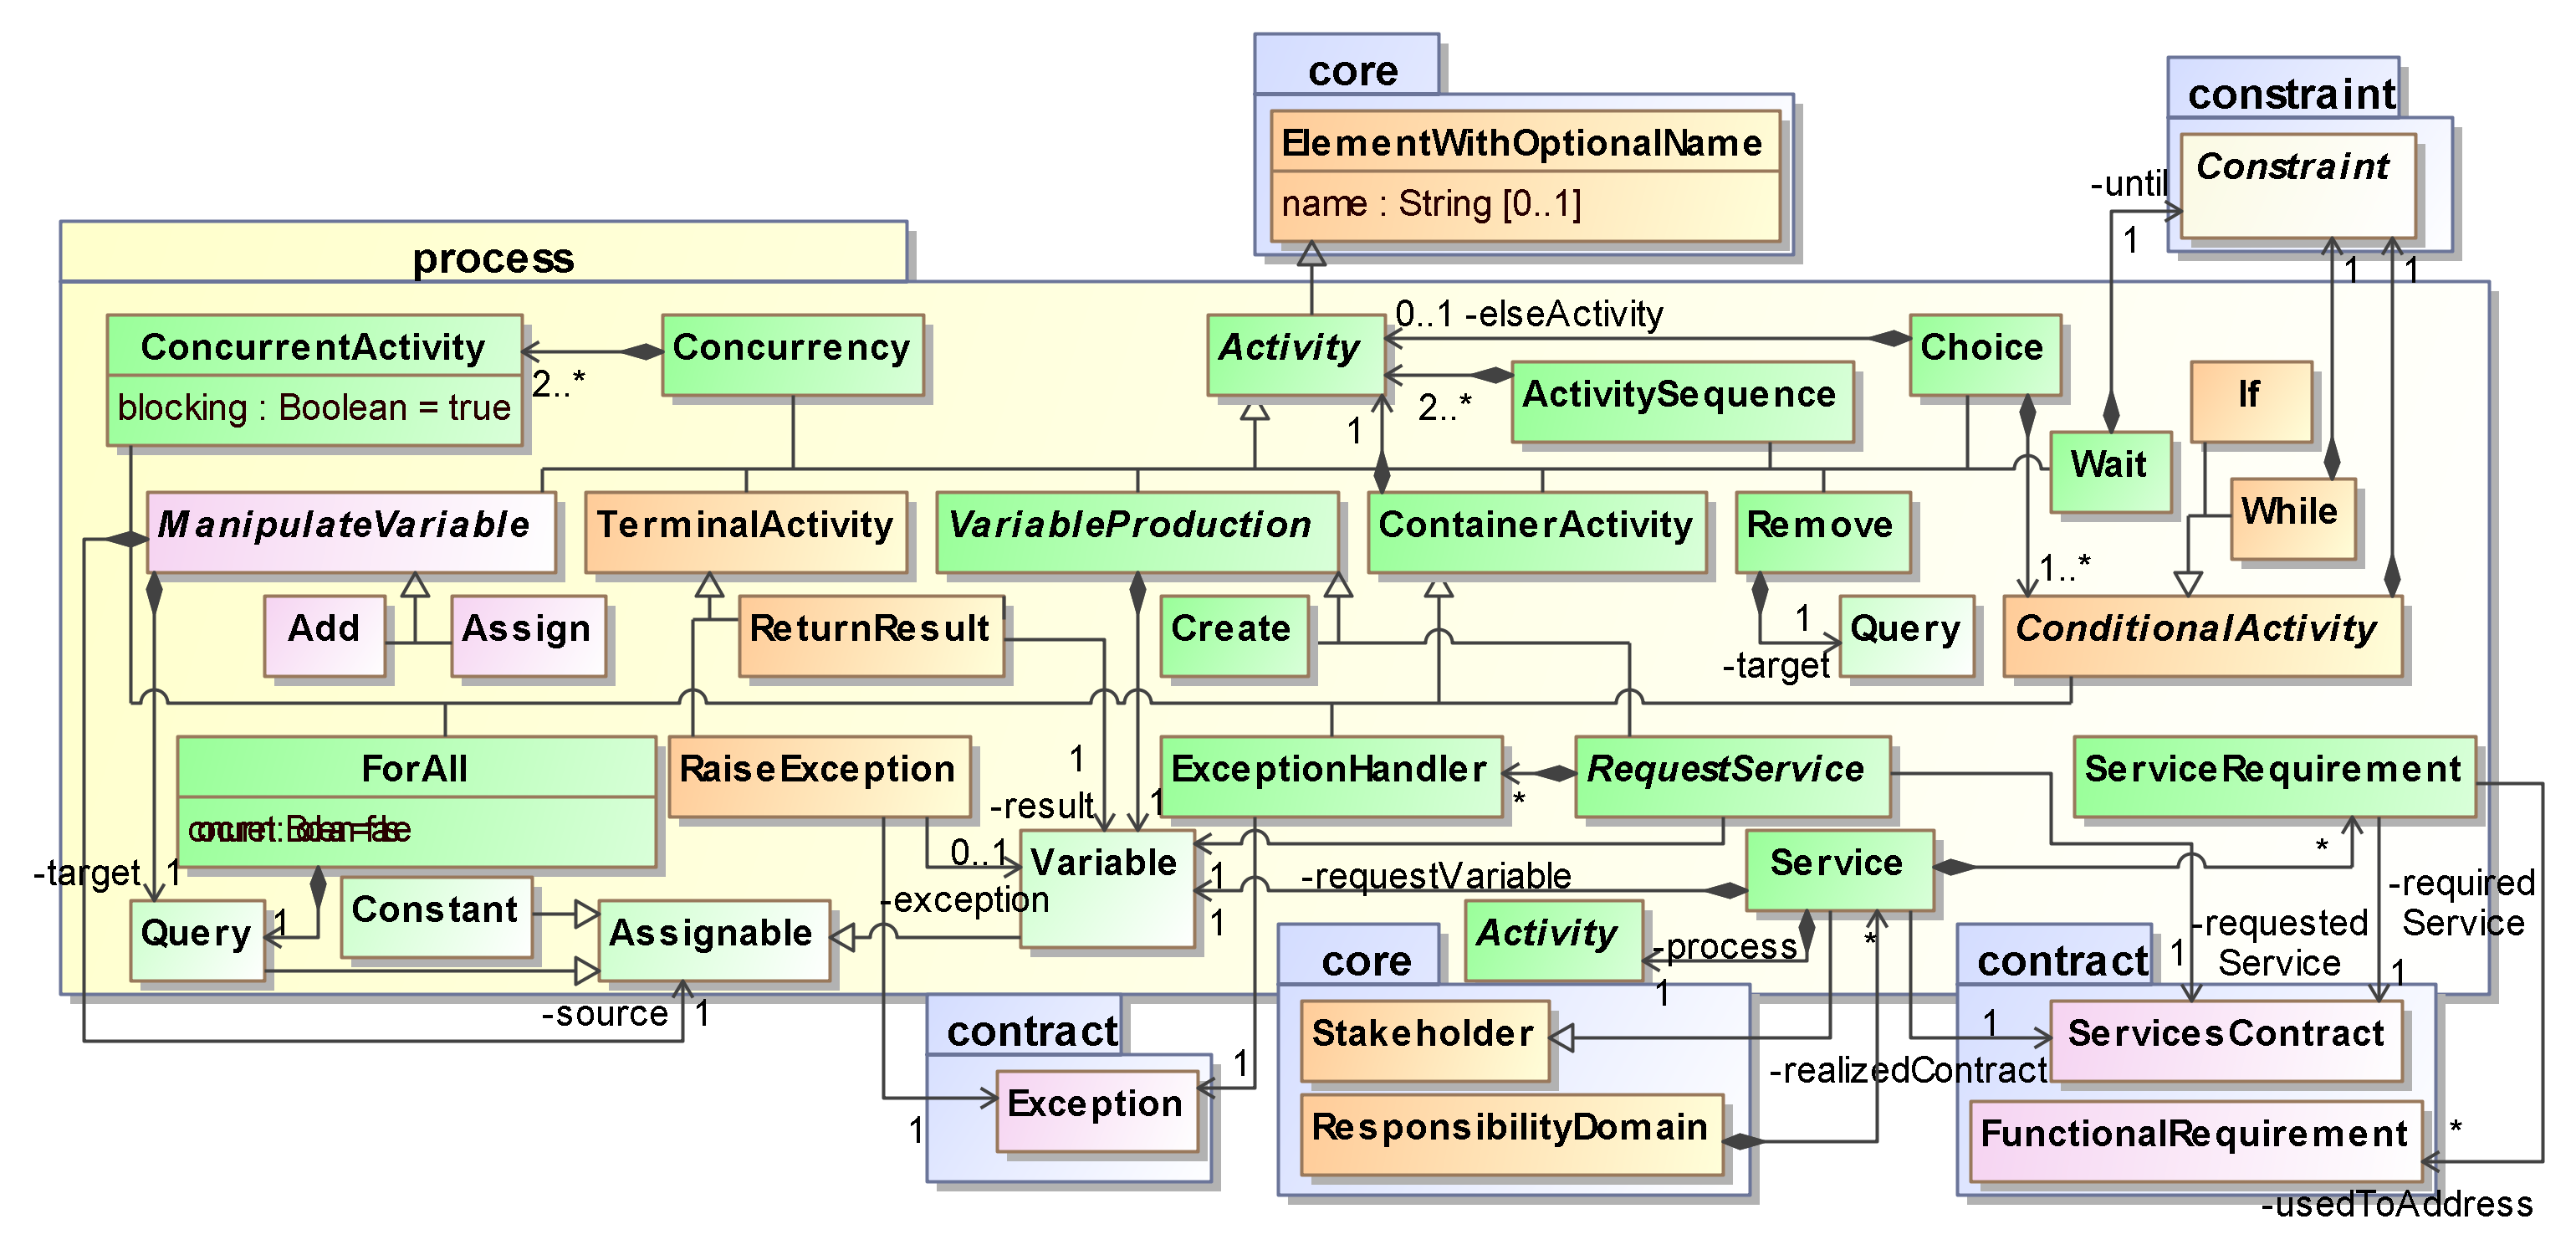
\includegraphics{process}
  \caption{The modeling constructs available for specifying services and processes in URDAD}
  \label{fig:processModule}
\end{figure}

Finally we use URDAD to design its analysis process. For this we use the URDAD modeling constructs for process specification shown in figure \ref{fig:processModule} (of course via the URDAD-DSL text grammar). Note that, following the URDAD process discussed in \ref{sec:urdad} we first specify the services we want to use to address each of the functional requirements (the \verb+usedToAddress+ links between a service requirement and a functional requirement represents the satisfaction links of \cite{ramesh_toward_2001}) before choreographing the process across these services. 

The following listing is an excerpt of the URDAD analysis process generated by applying URDAD to design the \verb+performAnalysis+ service:
\lstset{language=urdad,caption=Specifying the performAnalysis service in the textual URDAD DSL syntax.,label=serviceTextSyntax}
\begin{lstlisting}[numbers=left,escapechar=|]
Service provideServiceImpl realizes provideService receiving Variable provideServiceRequest ofType ProvideServiceRequest
{
  use provideServicesContract toAddress ( serviceContractSpecified serviceHasStakeHolders stakeholderRequirementsConsistent)
  use sourceService toAddress (serviceSourcedFromEnvironment)
  use designService toAddress (serviceSpecified)
        
  Process doSequential
  {
    create Variable provideServiceContractRequest ofType ProvideServiceContractRequest
    set Query OCL:"provideServiceContractRequest.serviceRequirements" equalTo Query OCL:"provideServiceRequest.serviceRequirements"
    requestService provideServiceContract with provideServiceContractRequest yielding Variable provideServiceContractResult ofType ProvideServiceContractResult raises (NoStakeholdersException InconsistentRequirementsException) 

    create Variable sourceServiceRequest ofType SourceServiceRequest
    set Query OCL:"sourceServiceRequest.serviceContract" equalTo Query OCL:"provideServiceContractResult.serviceContract"
    requestService sourceService with sourceServiceRequest yielding Variable sourceServiceResult ofType SourceServiceResult on NoRealizingServiceException
    doSequential
    {
      create Variable designServiceRequest ofType DesignServiceRequest
      set Query OCL:"designServiceRequest.serviceContract" equalTo Query OCL:"provideServiceContractResult.serviceContract"                
      requestService designService with designServiceRequest yielding Variable designServiceResult ofType DesignServiceResult
      forAll requiredService in Query OCL:"designServiceResult.service.requiredServices."
      {
        create Variable provideLowerLevelServiceRequest ofType ProvideServiceRequest
        add Query OCL:"requiredService" to Query OCL:"provideLowerLevelServiceRequest.serviceRequirements"
        requestService provideService with provideLowerLevelServiceRequest yielding variable provideLowerLevelServiceResult ofType ProvideServiceResult 
      } 
    } 
  }             
}
\end{lstlisting}

Comparing the above listing we see that \emph{performAnalysis} process corresponds to the original process discussed in section \ref{sec:urdad}.

\section{Related work \label{sec:relatedWork}}

The URDAD methodology provides a services-oriented methodology for generating a semi-formal analysis and design model representing MDA's PIM and supporting test and implementation generation. \cite{iacob_model-driven_2008} discuss an alternative approach. Business Rules are specified using OMG's {\em Semantics for Business Vocabulary and Rules} (SBVR) to service specification and orchestration and BPEL process specifications are generated using MDA tools. Processes are assembled from services which are related to business rules. This is similar to our satisfiability links specifying the services used to realize the different functional requirements.

The URDAD DSL allows for the specification of textual and graphical grammars through which the URDAD model is populated. An alternative approach is to define a separate metamodel for the use case narrative and to transform the narrative model requirements model \cite{hoffmann_towards_2009,osis_transforming_2010}. This approach introduces the complexities of having to transform from the narrative to the UML model and requires extensive consistency checks between the narrative and the UML models.

\cite{asnina_computation_2010} stress the need of modelling in the problem domain as well the benefits of accumulating requirements within a single model. Services are grouped into feature sets which are related to responsibility domains. Functional requirements are decomposed across levels of granularity and higher level processes are orchestrated across lower level services. They define the notion of functionals with cause and effect which can be related to the concept of a services contract. In addition they provide a {\em topological functional model} (TFM) for mapping technology neutral service requirements onto available concrete services pool. The TFM is independent of the modelling technique and can be applied to an URDAD model. 

In the {\em Requirements Driven Design Automation} methodology (RDDA) \cite{cardei_model_2008} one encodes requirements specifications in SYSML diagrams. The SYSML model is enriched with semantic descriptions after which the model is transformed to the {\em One Pass to Production} (OPP) design language, the ODL. ODL is an OWL based ontology from which the requirements are validated for consistency and completeness. The approach is, however, structure focused with little emphasis on services contracts and recursive orchestration of higher level services from lower level services.


\section{Conclusions and outlook}

In this paper we identified the stakeholders in the analysis and design methodology and the resultant requirements and technology neutral process design model and their quality requirements. We related these quality requirements to quality drivers and measures which can be applied within a services-oriented approach. We then identified that subset of quality drivers which has been embedded within the URDAD process and pointed out how some of these are enforced by the URDAD metamodel.

One of the practical benefits of the URDAD methodology is that it assists requirements engineers to make the paradigm shift\cite{haines_impact_2007} to defining stand-alone services contracts and to assemble processess from abstract, reusable, stateless services with the concrete service providers either selected during the implementation mapping phase or alternatively provided by the execution environment through mechanisms like real-time service provider selection and dependency injection.

Future work includes the specification of a graphical grammar making the domain specific language for URDAD accessible to requirements engineers like business analysts and the specification and development of quality assessment tools which can be used to either report quality measures or provide real time quality guidelines to modelers.

\bibliographystyle{plain}  %%abbrv
\bibliography{../../bibliography}

\end{document}
